\section{Results}\label{sec:results}
We quantify the Jao Gap location along the magnitude axis by first subsampling
our synthetic populations, finding the linear number density along the
magnitude axis of each subsample, averaging these linear number density and
extracting peaks from this above a prominence threshold.w Once we have the peak
location we fit a gaussian to a window centered at the peak giving both an
estimate of the gap location and the gap width. Figure \ref{fig:JaoGapLocator}
shows this fit for both OPAL and OPLIB populations.

\begin{table}
	\centering
	\begin{tabular}{c | c c}
		\hline
		Model & Location & Prominence \\
		\hline
		\hline
		OPAL & 10.15864 & 0.19501 \\
		OPLIB 1 & 10.17813 & 0.26055 \\
		OPLIB 2 & 10.21313 & 0.46898
	\end{tabular}
	\caption{Locations identified as potential gaps.}
	\label{tab:GapLocation}
\end{table}

Our gap identification method finds two potential gaps in the OPLIB (Table
\ref{tab:GapLocation}) data while only finding one in the OPAL dataset. This
apparent discrepancy is not due to a fundamental structural difference between
the OPAL and OPLIB opacity tables; rather, it is attributable to the the
phasing of the periodic luminosity variations seen accorss mass in Figures
\ref{fig:OPALPunchIn} and \ref{fig:OPLIBPunchIn} and whether or not the
injected noise smears all of these together into one gap or two gaps.
{\color{red} [Run a test where you manually shift the OPAL data to the same
phase as the OPLIB data to show that this has the effect of making two gaps
show up]}.

\begin{figure}
	\centering
	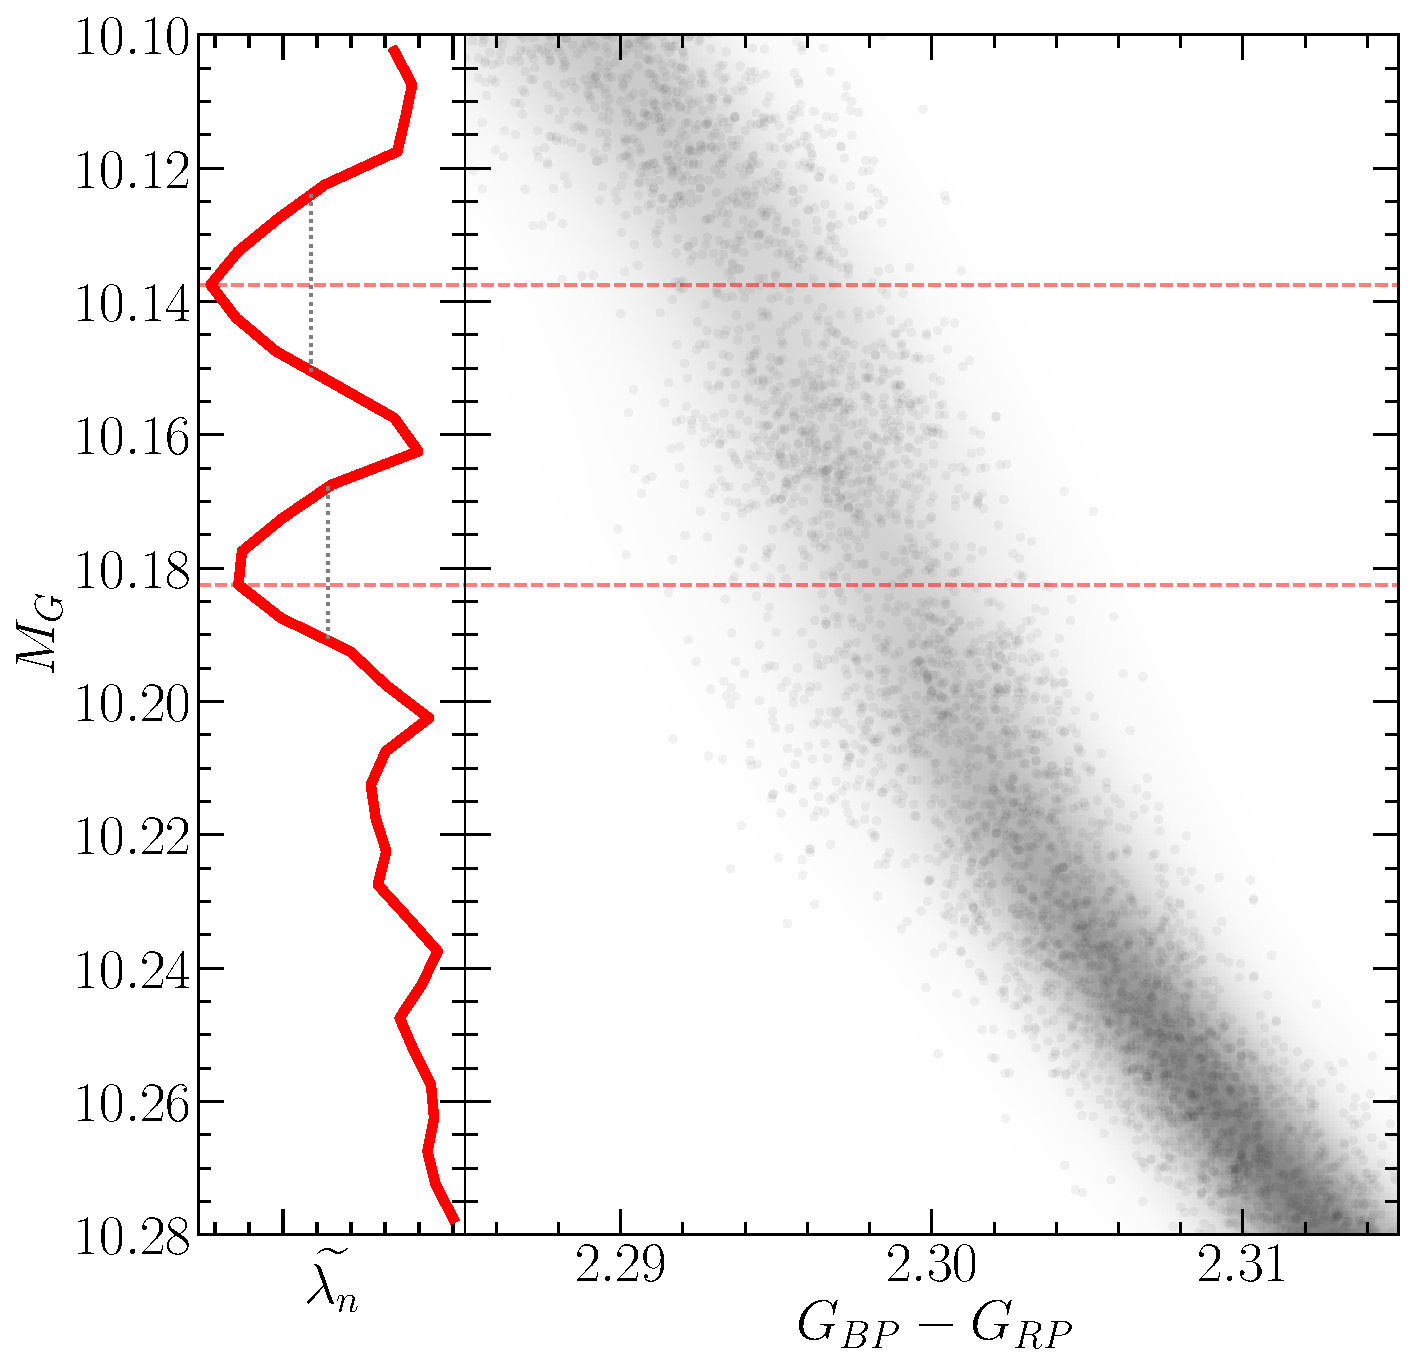
\includegraphics[width=0.45\textwidth]{src/figures/NotebookFigs/OPAL_Jao_locator.png}
	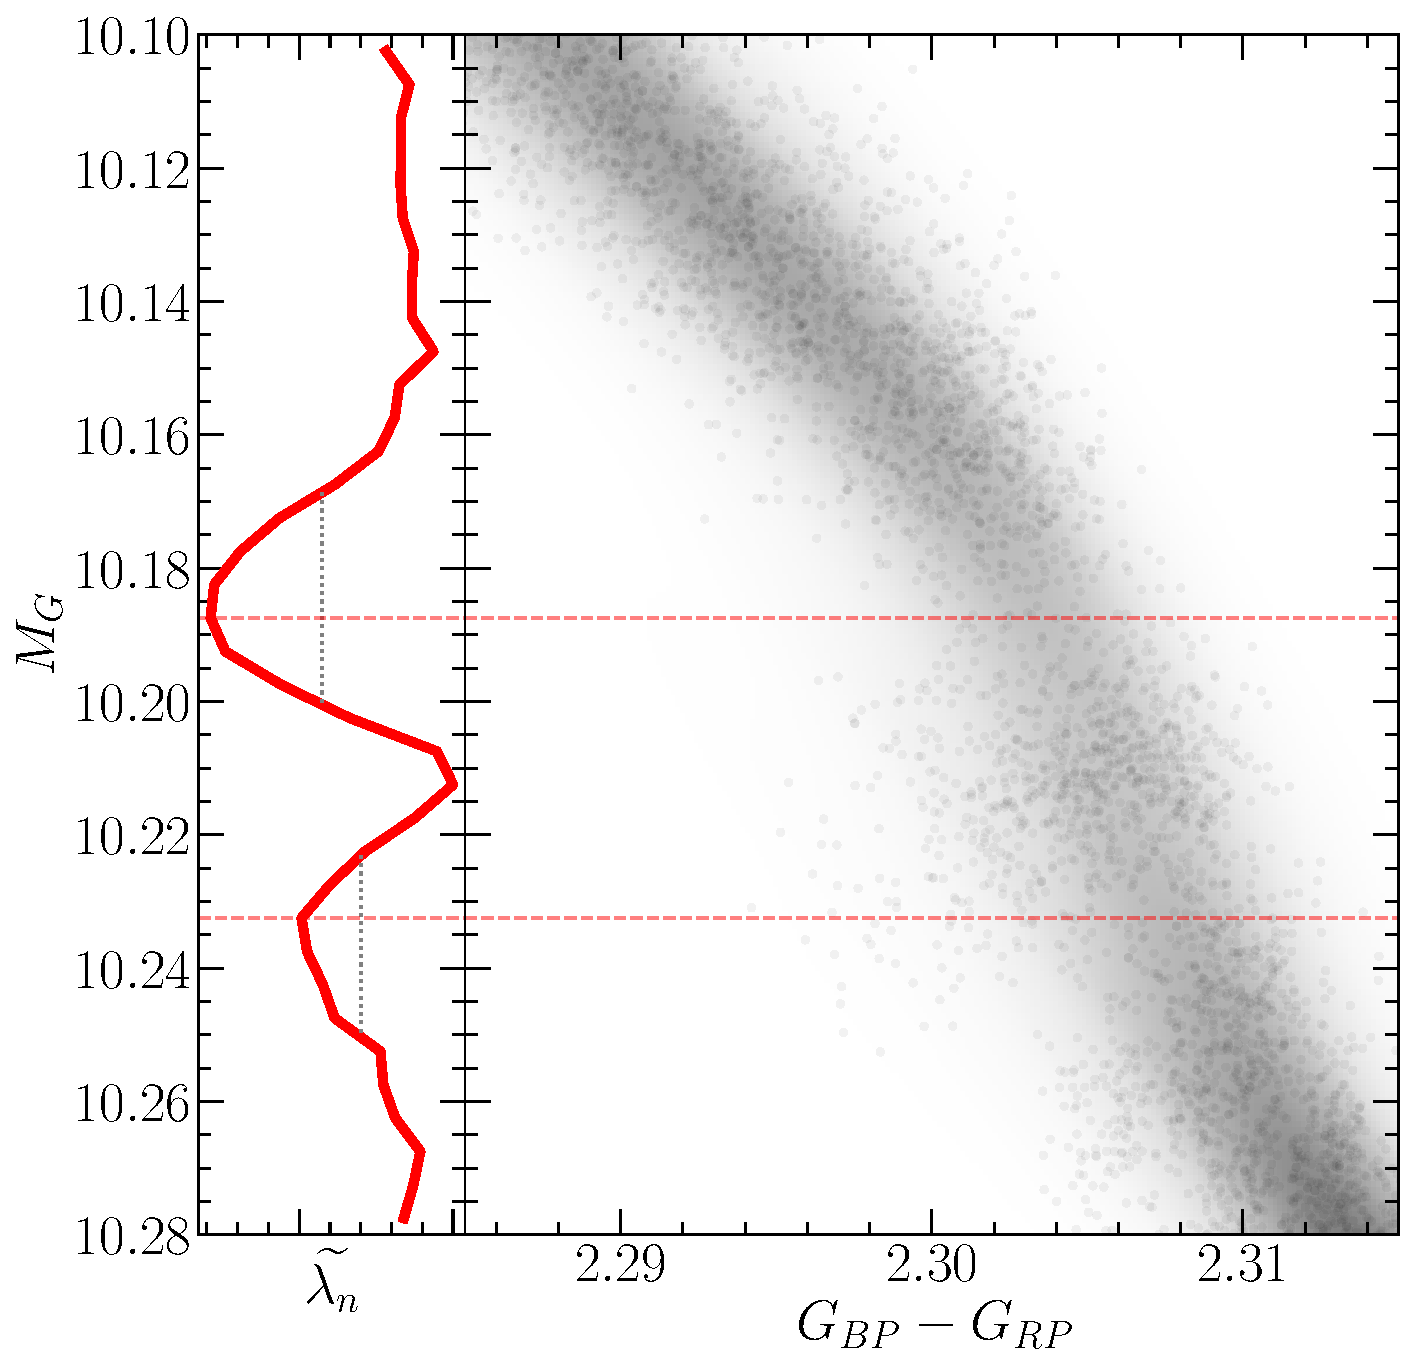
\includegraphics[width=0.45\textwidth]{src/figures/NotebookFigs/OPLIB_Jao_locator.png}
	\caption{(right panels) OPAL (top) and OPLIB (bottom) synthetic
	populations. (left panels) Normalized linear number density along the
	magnitude axis. A dashed line has been extended from the peak through both
	panels to make clear where the Identified Jao Gap location is wrt. to the
	population. }
	\label{fig:JaoGapLocator}
\end{figure}

Both gaps identified in the OPLIB sample are at fainter magnitudes than the gap
identified in the OPAL sample. This implies that in the OPLIB sample the
convective mixing events which drive the kissing instability should happen more
regularlry and therefore also start earlier in the models evolution. This is
because each mixing event serves to interupt the ``standard'' luminosity
evolution of a stellar model, kicking its luminosity back down to what it would
have been a few Gyrs earlier instead of allowing it to slowly increase. Looking
at the interior physics of one OPAL and one OPLIB model shows that this shorter
duration between mixing events is in fact seen (Figure {\color{red} [PUT
KIPPENHAN DIAGRM HERE]}.

The slightly lower opacities charectaristic to OPLIB serve to shallow the
radiative temperature gradient, $\nabla T_{rad}$; however, as the adiabatic
temperature gradient remains essentially unchanged, a larger interior radius of
the model will remain unstable to convection {\color{red}[CHECK IF THIS OR IF
RADIATIVE ZONE MOVING IN]}. This larger convective zone and therefore smaller
radiative zone is in line with the behavior of the models presentd here. We see
that OPLIB models undergo convective mixing events earlier in their evolution
than OPAL models (Figure \ref{fig:OPALOPLIB3He} implying that the inner
convective zone did not have to expand as much to meet the outer convective
zone. 

\begin{figure}
	\centering
	\includegraphics[width=0.45\textwidth]{src/figures/NotebookFigs/3HeOPAL_OPLIB.pdf}
	\caption{Core $^{3}$He mass fraction for a model evolved with OPAL and a
	model evolved with OPLIB within the Jao Gap's mass range. Note how the
	OPLIB model undergoes the mixing event earlier in its evolution than the
	OPAL model does.}
	\label{fig:OPALOPLIB3He}
\end{figure}

{\color{red} Then compare the results to observations, comment on which one
matches observations better and also how confident we can be about that}

{\color{red} Comment on if the shift in the gap location is larger or smaller
than the size o fthe gap or the shift due to other effects such as variations
in age or composition, i.e is it Significant enough to matter}

{\color{red} comment on why the gap shifts in the manner which it does, i.e the
opacities are lower. Show how for a constant opacity table increasing the
metallicity (which will also change the opacity) affetcs the gap location)}
